% !TEX root = ../../../main.tex
% 来源：中学数学实验教材·第二册（几何）
% 章节：直线形 / 三角形
% 原始文件：3.tex，行 735-741
% 类型：tikz
% ---
    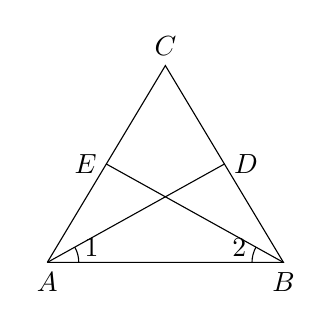
\begin{tikzpicture}[>=latex, scale=1]
\draw(-1.5,0)node[below]{$A$}--(0,2.5)node[above]{$C$}--(1.5,0)node[below]{$B$}--(-1.5,0);
\draw(-.75,1.25)node[left]{$E$}--(1.5,0);
\draw(.75,1.25)node[right]{$D$}--(-1.5,0);
\draw(-1.5+.4,0) arc (0:29:.4)node[right]{1};
\draw(1.5-.4,0) arc (180:180-29:.4)node[left]{2};
    \end{tikzpicture}
